\chapter{Inhalt}

\section{Spülenkonzepte}
Man unterscheidet zwischen Ein- und Mehrbecken-Spülen. Letztere verfügen über ein kleineres Zusatzbecken und/oder ein zweites vollwertiges Hauptbecken, um parallele Arbeitsgänge wie das Ausgießen von Resten oder das Waschen von Gemüse zu ermöglichen. Da die meisten Haushalte über einen Geschirrspüler verfügen, ist zum komfortablen Reinigen größerer Gegenstände, z. B. Backblechen, Schneidbrettern oder Woks, ein geräumiges Hauptbecken mit großer Beckendiagonale besonders vorteilhaft. Häufig werden Spülbecken mit einer Abtropffläche[1] kombiniert, um abtropfendes Wasser in das Spülbecken zurückzuführen.

Rundbecken-Spülen sind zumeist als Einbecken-Spülen mit vergleichsweise kleinen Spülbecken konzipiert. Eckspülen sind spezielle Lösungen für Eckunterschränke. \cite{moore}\cite{MopOverview}

Spülbecken müssen in Deutschland mit einem Überlauf ausgestattet sein, um dem versehentlichen Fluten der Küche vorzubeugen; in anderen Staaten sind auch Spülen ohne Überlauf zugelassen.\cite{scala}\cite{rltl}

Für die Gastronomie sind Spülbecken in der DIN 66075-5 (Gastro-Norm: Einrichtungen für die Gastronomie; Spülbecken, Maße; Ausgabe 1975-07) genormt.


\section{Materialien}
Edelstahl ist der populärste Werkstoff für Spülbecken, der seit den 1950er Jahren in verschiedenen Material-Spezifikationen (z. B. DIN 1.4301) zum Einsatz kommt. Neben der klassischen glatten Oberfläche in unterschiedlichsten Veredelungen werden auch Spülen aus geprägtem Edelstahl, z. B. mit Leinen-Struktur, angeboten, die die Empfindlichkeit des Materials gegenüber Kratzern halbwegs kaschiert. Die Produktion von einfacheren Edelstahl-Spülen erfolgt durch Tiefziehen von Edelstahlblechen, anspruchsvollere Produkte entstehen durch Zusammenfügen mehrerer tiefgezogener Komponenten, aber auch durch Verschweißen von Blechzuschnitten. \cite{bitkom}\cite{Leucker02}

Seit Beginn der 1980er Jahre gibt es Küchenspülen aus hochwertigen Verbundwerkstoffen. Sie werden in vielen Farben und Formen angeboten. Hochwertige Produkte sind zumeist ausgesprochen kratzfest und pflegeleicht und halten Temperaturen bis 280 °C sowie allen küchenüblichen Beanspruchungen (z. B. stark färbende Lebensmittel oder Säuren) stand. Moderne Produktionsverfahren ermöglichen auch filigrane Formen, die mit anderen Werkstoffen nicht zu realisieren sind.

Keramik und Steinzeug sind traditionelle Werkstoffe, die seit vielen Jahrzehnten auch für die Herstellung von Küchenspülen eingesetzt werden.
Keramik-Spüle mit Zusatzbecken, Tropffläche, umhängbarer Edelstahl-Schale und verschiebbarem Schneidbrett aus Sicherheitsglas

Ein ebenfalls früher häufiger verwendeter Werkstoff ist Terrazzo, der heute jedoch nur noch für besonders exklusive Becken verwendet wird. Nachteilig ist das verhältnismäßig große Gewicht, das eine entsprechend stabile Unterkonstruktion nötig macht.

Naturstein ist als Material für Spülbecken weitgehend bedeutungslos geworden da viele Steinmaterialien nicht widerstandsfähig genug sind (z. B. Marmor) oder nicht mehr heutigen hygienischen Ansprüchen entsprechen (z. B. der Flüssigkeiten aufsaugende Sandstein).

Glas wird zumeist mit anderen Werkstoffen kombiniert. In den meisten Fällen werden Edelstahl-Becken mit einem horizontalen Arbeitsbereich aus Glas verbunden. \cite{RltlConv}

Emaillierter Stahl hat als Spülen-Werkstoff nur noch geringe Bedeutung. Er steht für die Anfänge farbiger Küchen-Spülen, die seit den Achtziger Jahren durch komfortablere und strapazierfähigere Produkte aus Verbundwerkstoff oder farbiger Keramik verdrängt wurden. \cite{codecommit}


\begin{figure}[ht]
	\centering
  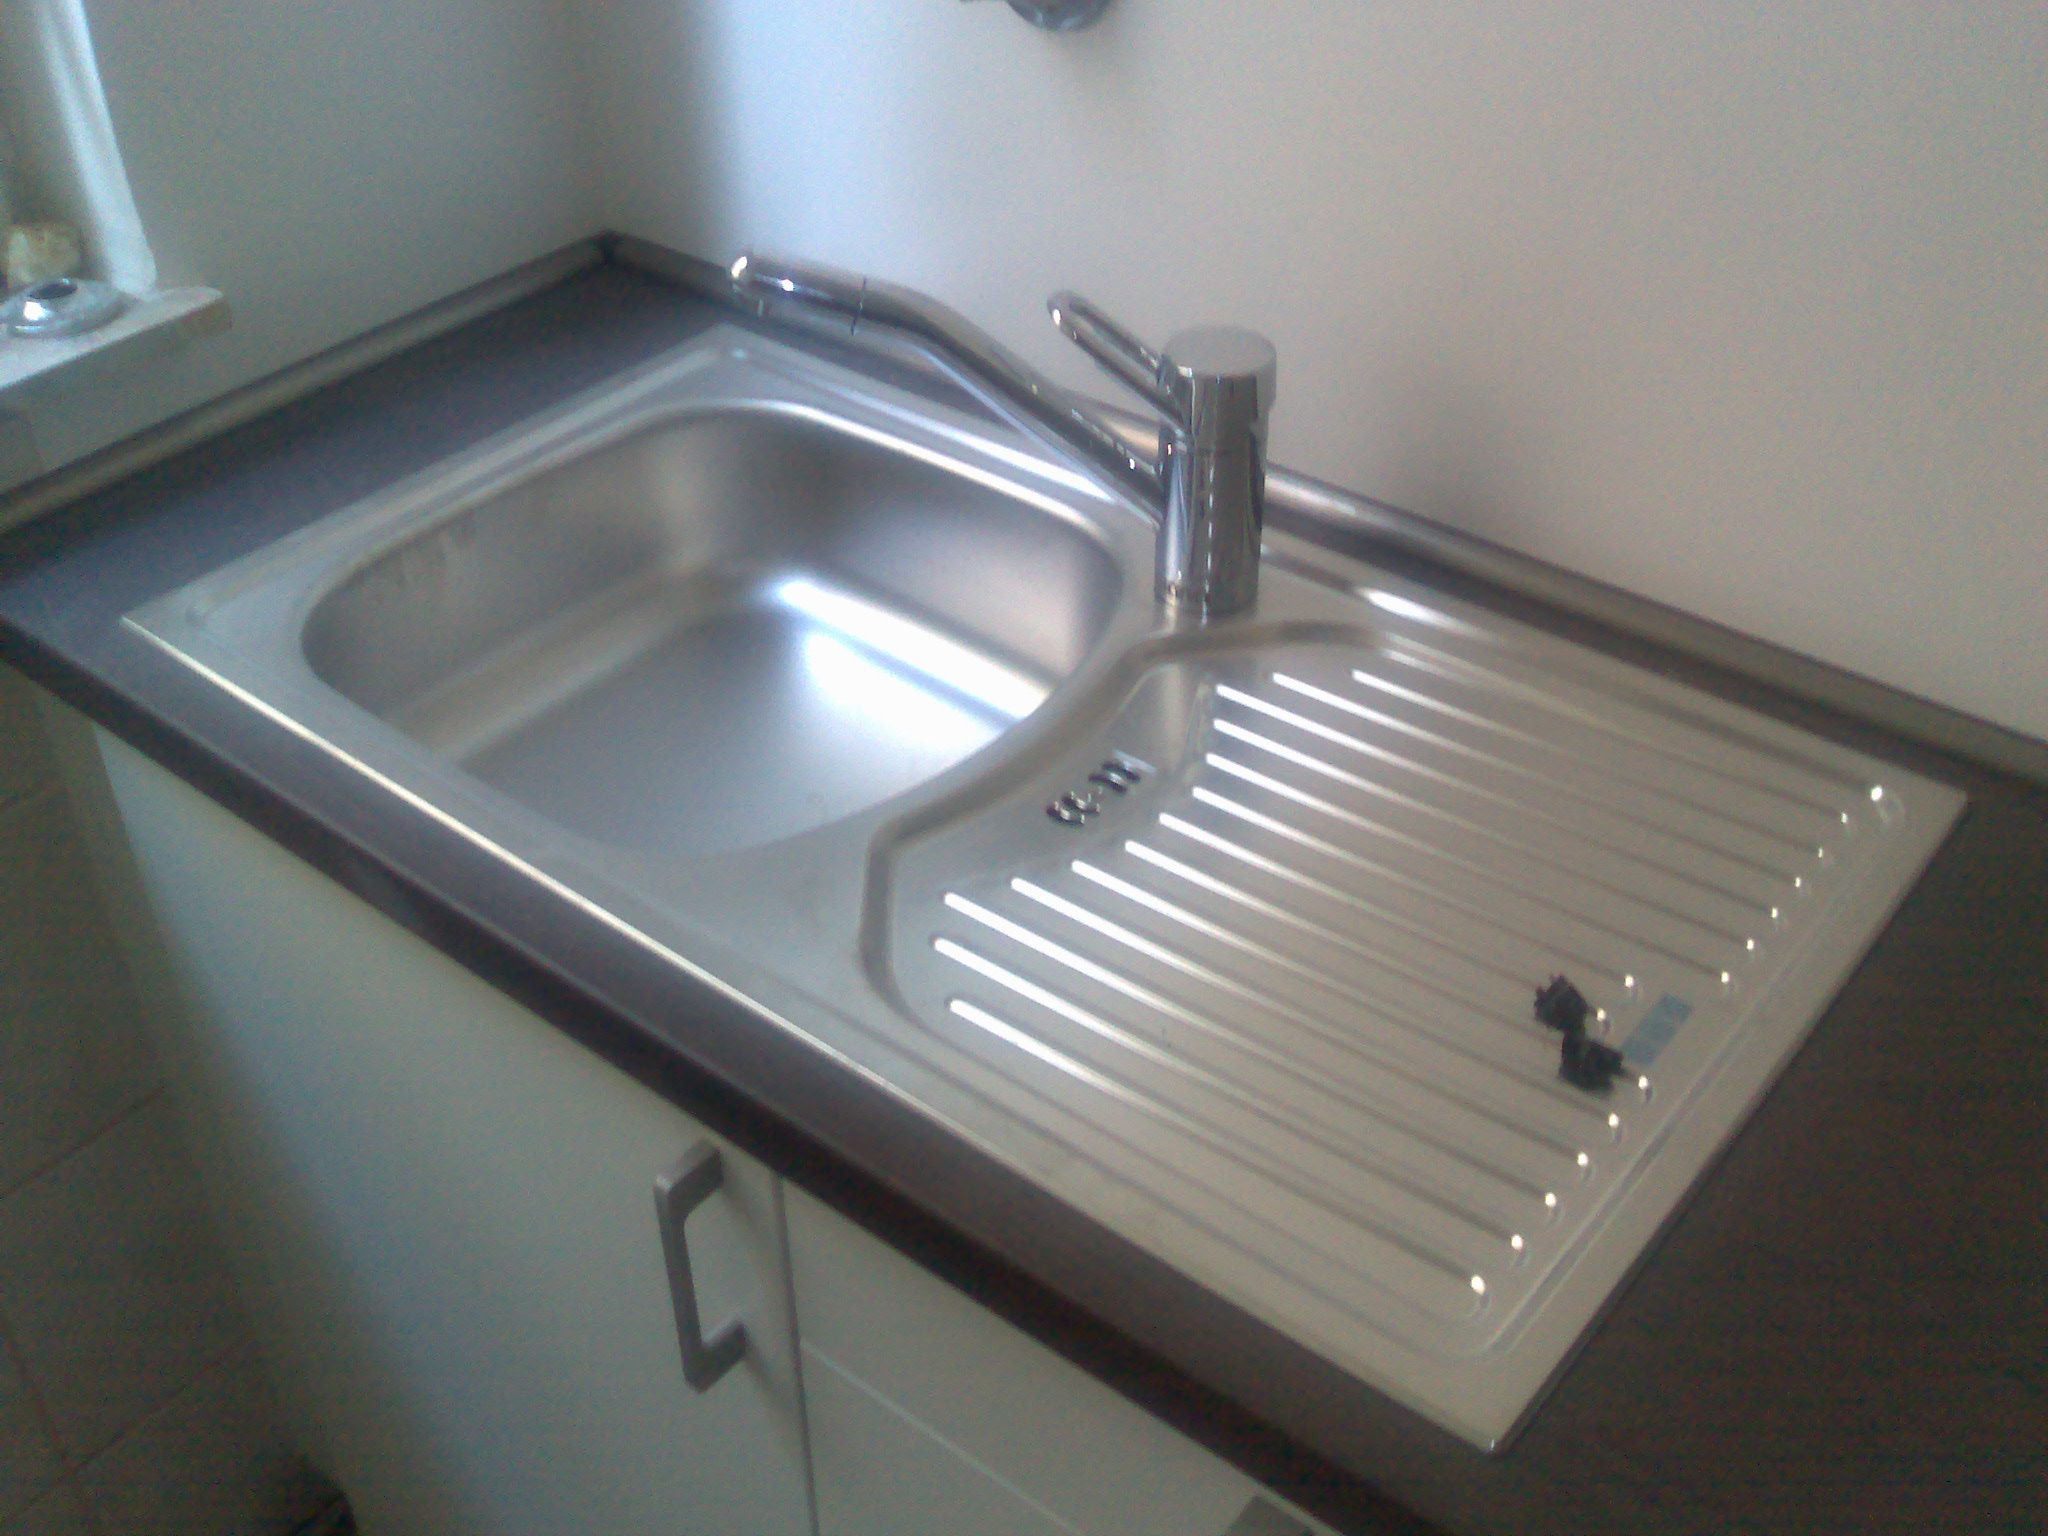
\includegraphics[width=0.9\textwidth]{Spuelbecken.jpg}
	\caption{Spülbecken mit Abtropffläche}
	\label{fig1}
\end{figure}


\begin{figure}[ht]
	\centering
  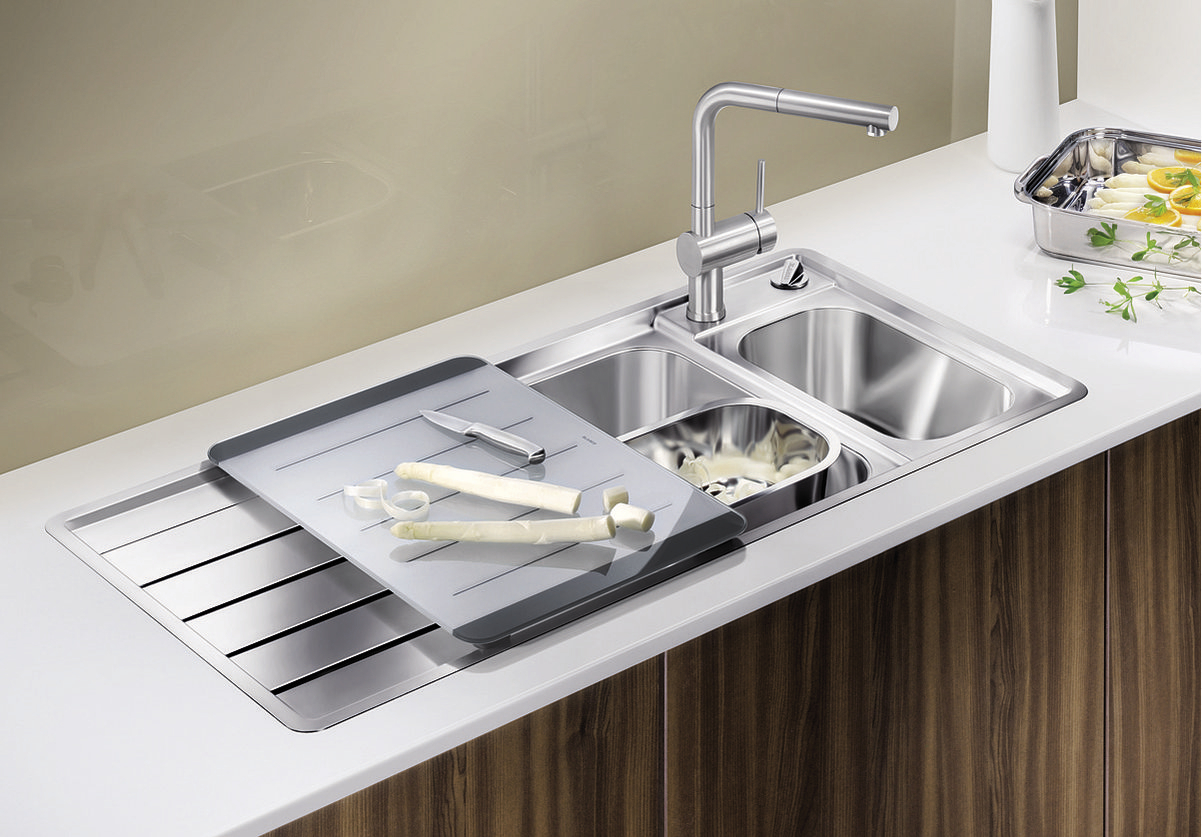
\includegraphics[width=0.9\textwidth]{Spuelbecken2.jpg}
	\caption{
Edelstahl-Spüle mit Zusatzbecken, Tropffläche und verschiebbarem Schneidbrett aus Sicherheitsglas}
	\label{fig1}
\end{figure}
